\documentclass[conference]{IEEEtran}
\IEEEoverridecommandlockouts

\usepackage{cite}
\usepackage{amsmath,amssymb,amsfonts}
\usepackage{algorithmic}
\usepackage{graphicx}
\usepackage{textcomp}
\usepackage{xcolor}
\usepackage{hyperref}
\usepackage{multicol}
\usepackage{multirow}
\usepackage{orcidlink}
\usepackage{tabularx}
\usepackage{lscape}
\usepackage{tikz,xcolor,hyperref}
\usepackage[normalem]{ulem}
\usepackage{tabularray}
\renewcommand{\arraystretch}{1.5}
\usepackage{caption}
\captionsetup[figure]{font=small}
\usepackage{etoolbox}
\makeatletter
\patchcmd{\@makecaption}
  {\scshape}
  {}
  {}
  {}
\makeatother

% Đặt màu cho url
\hypersetup{
    colorlinks=true,
    linkcolor=blue,
    filecolor=magenta,      
    urlcolor=blue,
    }
\definecolor{lime}{HTML}{A6CE39}

% Orcid ID
\DeclareRobustCommand{\orcidicon}{
	
\begin{tikzpicture}
	\draw[lime, fill=lime] (0,0) 
	circle [radius=0.16] 
	node[white] {{\fontfamily{qag}\selectfont \tiny ID}};
	\draw[white, fill=white] (-0.0625,0.095) 
	circle [radius=0.007];
	\end{tikzpicture}
	\hspace{-2mm}
}
\foreach \x in {A, ..., Z}{\expandafter\xdef\csname orcid\x\endcsname{\noexpand\href{https://orcid.org/\csname orcidauthor\x\endcsname}
			{\noexpand\orcidicon}}
}
\newcommand{\orcidauthorA}{0009-0001-3187-4144}
\newcommand{\orcidauthorB}{0009-0004-3101-4840}
\newcommand{\orcidauthorC}{0000-0002-3614-7982}
\newcommand{\orcidauthorD}{0000-0003-3046-3041}

\def\BibTeX{{\rm B\kern-.05em{\sc i\kern-.025em b}\kern-.08em
    T\kern-.1667em\lower.7ex\hbox{E}\kern-.125emX}}

\renewcommand\thesection{\Roman{section}}
\renewcommand\thesubsection{\thesection.\arabic{subsection}/}

% TODO: làm sao để có đường gạch ngang trên footnote



\begin{document}
\title{Enhanced Image Captioning using\\Efficient Pretrained Word Embedding\\}
% TODO: thêm thầy
\author{\IEEEauthorblockN{Quang-Huy Nguyen\orcidA, Hoai-Phong Le\orcidB,  Xuan-Nam Cao \orcidC, Minh-Triet Tran \orcidD}
\IEEEauthorblockA{\textit{Falcuty of Information Technology, University of Science, VNU-HCM} \\
\textit{Vietnam National University, Ho Chi Minh City, Vietnam}\\
20120497@student.hcmus.edu.vn, 20120545@student.hcmus.edu.vn}
}
\maketitle

\begin{abstract}
% Giới thiệu IC
Image captioning is an interesting and challenging problem at the intersection of computer vision and natural language processing.
% giới thiệu vấn đề
One of the most significant breakthroughs of natural language processing is the use of vector representations for words, representing them as numerical vectors rather than as sequences of characters. These representations can be trained as task-specific or pretrained using a large corpus of text. However, in the context of image captioning, the use of pretrained word embeddings has not been widely explored.
% What question
In this paper, we investigate the impact of pretrained word embeddings on the quality of an image captioning model. Specifically, we focus on ResNet-50 and LSTM with a soft attention mechanism approach and experiments with three different word embeddings: non-pretrained, pretrained fastText, and pretrained GLoVe. The evaluation is conducted on the Flickr30k dataset, which comprises 31,000 images, each associated with five captions.
% Result
We report that the BLEU-4 scores obtained are 0.2407 for the non-pretrained embedding, 0.2412 for fastText, and 0.2475 for GLoVe. The results indicate that both fastText and GLoVe embeddings enhance the model's ability to generate more accurate and contextually relevant captions. Overall, this work demonstrates that using pretrained word embeddings slightly improves the performance of the captioning model, with GLoVe embeddings being particularly well suited for this image captioning task.
% TODO: non-pretrained || no pretrained || no pretrained ???
\end{abstract} 

\begin{IEEEkeywords}
Image captioning, word embedding, fastText, GLoVe
\end{IEEEkeywords}

\section{Introduction}
% EN
% Độ phổ biến. Khái niệm. Ứng dụng
Image captioning is a challenging and meaningful domain of study that has attracted extensive research. It takes an image as an input and generates a textual description of the image as the output. Image captioning has many real-world applications, including human-computer interaction \cite{li2020oscar, zhang2021vinvl}, medical image captioning \cite{huang2021contextualized, karoly2006psychological}, quality control in industry \cite{luo2019visual}, image search engines \cite{iyer2019image}, and assistive technologies for visually impaired individuals \cite{dognin2020image, kim2021proceedings, yu2023quality}. Owing to its practical significance, there is a pressing need for continuous improvements in image captioning models.


% Sự thách thức
A quick glance at an image enables a human to effortlessly identify and describe an immense amount of details in the visual scene \cite{fei2007we}. However, image captioning has long been regarded as a difficult problem in computer science because it necessitates the integration of two major fields of Artificial Intelligence \cite{rinaldi2023automatic}: Computer Vision \cite{ijjina2016hybrid, wang2015feedforward} and Natural Language Processing \cite{cho2014learning, collobert2008unified}. 


% Sự thách thức
The task requires the model to not only accurately identify objects within images but also to comprehend the interactions and relationships between these objects to generate meaningful captions. Determining the presence, attributes, and relationships of objects in an image is not an easy task itself. Generating a human-like sentence to describe such information makes this task even more difficult \cite{bai2018survey}.


% Các phương pháp truyền thống
% In the early stages of image captioning research, traditional methods focused on using handcrafted features and rule-based approaches. For example, Kojima et al. \cite{kojima2002natural} used concept hierarchies of actions, verb patterns, and case structures to generate captions for human activities. Kuznetsova et al. \cite{kuznetsova2014treetalk} proposed a novel tree-composition approach for generating expressive image descriptions. Although these methods demonstrate basic captioning capabilities, they lack the ability to produce diverse and contextually relevant descriptions.


In the early stages of image captioning research, traditional image captioning approaches often rely on feature extraction methods, such as Histogram of Oriented Gradients (HOG) \cite{tomasi2012histograms}, Scale Invariant Feature Transform (SIFT) \cite{david2004distinctive}, Local Binary Patterns (LBP) \cite{ojala2000gray}, and Bag of Words (BoW) \cite{tsai2012bag}. These methods have demonstrated impressive results and have become popular in the field for many years. However, with the complexities involved in feature extraction, traditional methods are now less favored than deep learning-based approaches, which have the ability to automatically learn features from large datasets \cite{pouyanfar2018survey}.

\begin{figure}[t]
\centering
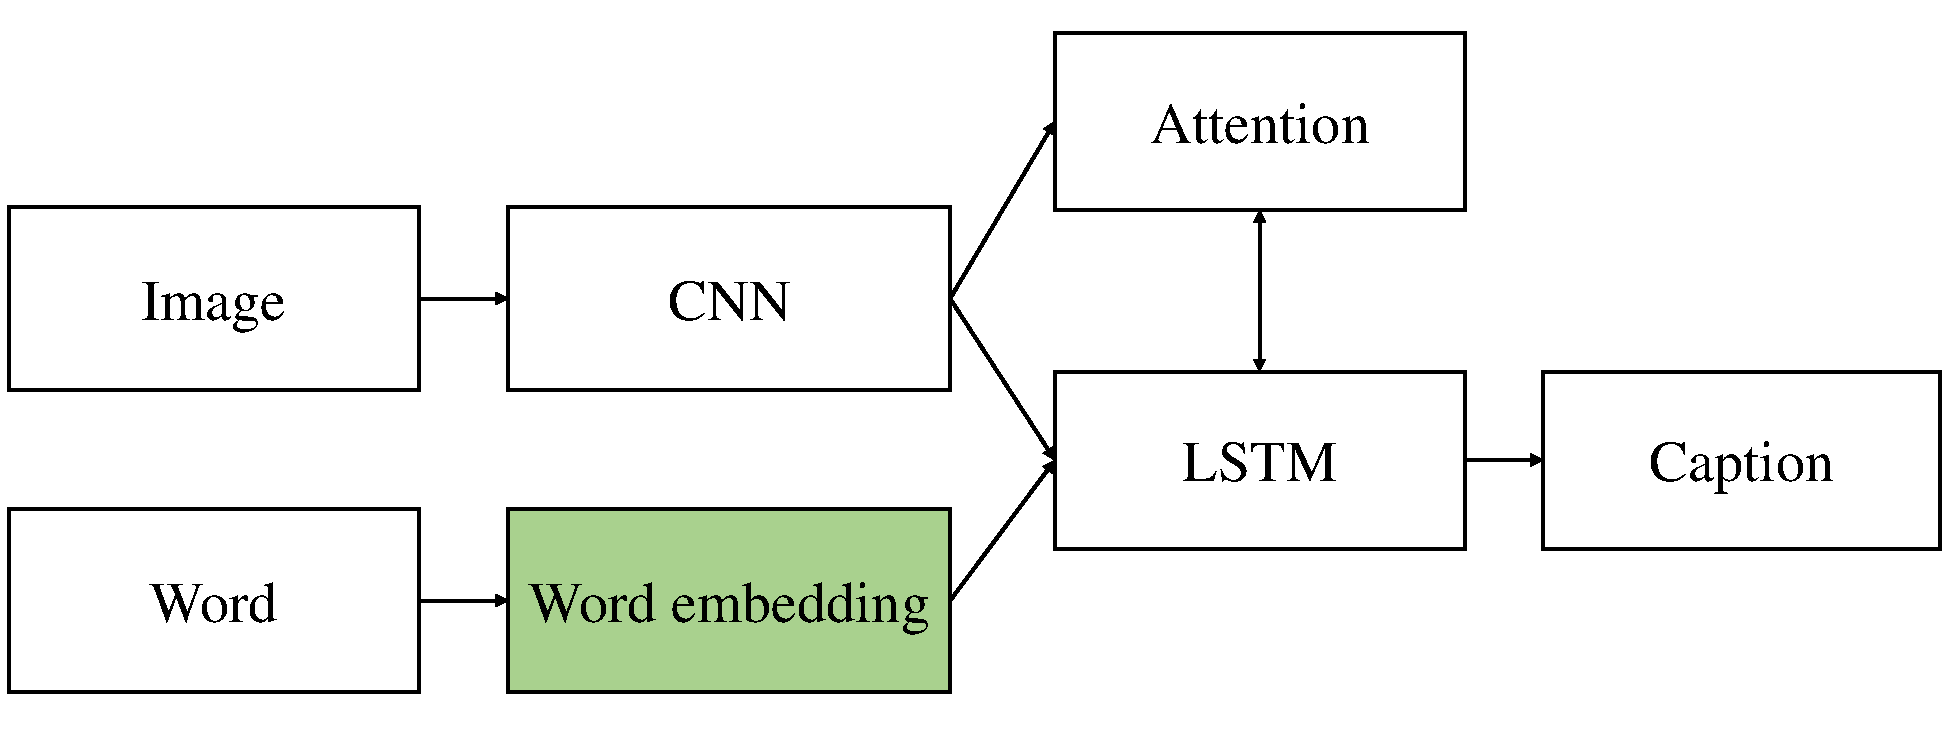
\includegraphics[width=0.95\columnwidth]{assets/abstract-architecture.pdf}
  \caption{Block diagram of an image captioning model using an encoder-decoder framework with an attention mechanism. This paper uses this architecture and focuses on Word embedding block.}
  \label{fig:example}
\end{figure}

\begin{figure}[t]
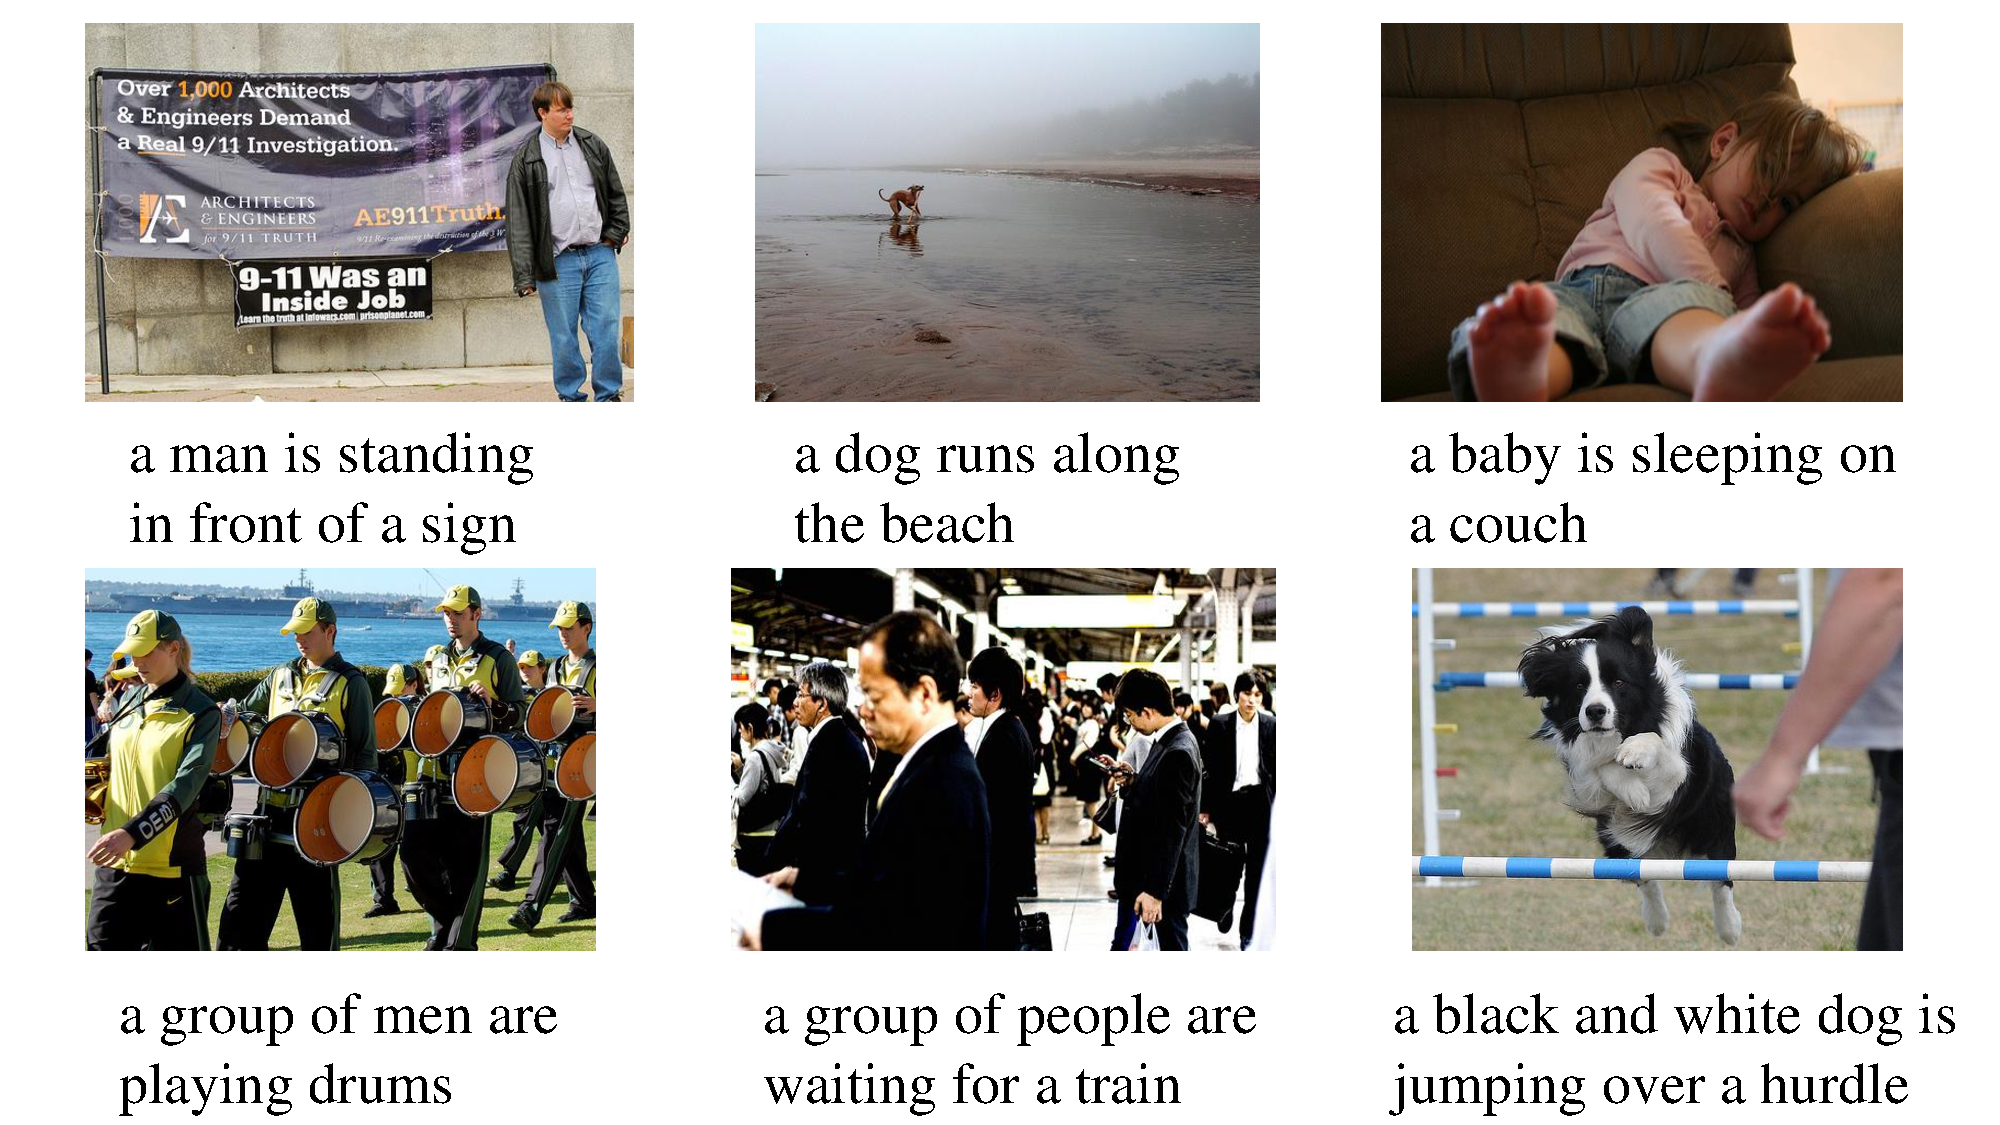
\includegraphics[width=\columnwidth]{assets/example_image_captioning.pdf}
\caption{Examples of captions for given images. These captions are generated using the proposed model with GloVe pretrained word embedding.}
  \label{fig:example}
\end{figure}


% Các phương pháp học sâu
The rapid advancement of deep learning \cite{krizhevsky2017imagenet, bengio2013representation, lecun2015deep} has revolutionized image captioning using data-driven neural network approaches. % TODO: Câu trước câu sau không liền nhau
Encoder-decoder models have been widely used in image captioning \cite{xiao2019deep}. Convolutional Neural Networks (CNNs) \cite{kim2014convolutional, lecun1995convolutional, Atliha2020} are employed as encoders to extract visual features from images, whereas Recurrent Neural Networks (RNNs) \cite{pascanu2013construct} or variants such as Long Short-Term Memory (LSTM) \cite{karpathy2015visualizing} and Gated Recurrent Units (GRU) \cite{do2020reference} serve as decoders for language sequences. This powerful combination helps the model generate descriptive and contextually relevant captions for diverse visual content.


% Cơ chế attention
At each step of the decoder's word generation process, it is unnecessary to consider information from the entire image; only information from the relevant regions is sufficient. This idea was proposed by Xu et al. \cite{xu2015show}, and it led to the introduction of the Attention mechanism \cite{niu2021review}. It enables the model to focus on the necessary regions of the image during each word-generation step, thereby enhancing the accuracy of the model. Additionally, the Attention mechanism improves the interpretability of the model \cite{gao2021interpretable}, allowing us to visualize the regions of the image that the model focuses on during the caption generation process.


% Cải tiến khác: pretrained
% Recent research has explored new novel approaches, including reinforcement learning \cite{kaelbling1996reinforcement}, multimodal fusion techniques \cite{zhao2019multimodal, kalimuthu2021fusion}, and the incorporation of external knowledge bases \cite{wu2017image}. They can enhance the image captioning performance. Moreover, transfer learning \cite{degadwala2021image} has been leveraged to fine-tune models pretrained on large-scale datasets, leading to improved generalization and efficiency.


% Embedding
To generate word sequences, whether using RNNs or transformers \cite{vaswani2017attention}, all methods operate not on sequences of characters, but at a higher level of abstraction, representing words as vectors of numbers. These vectors can be pre-associated with each word or adjusted during model training. Several techniques exist for establishing correspondence between words and numeric vectors. While one-hot encoding \cite{rodriguez2018beyond} is a straightforward approach, more sophisticated methods, % TODO: dùng từ hơi lạ lẫm
such as Word2vec \cite{mikolov2013efficient} or GLoVe \cite{pennington2014GLoVe}, have been developed.


% Nói về công việc trong nghiên cứu này
In the context of image captioning, pretrained vector representations for words have not been widely utilized because models are usually trained from scratch during the training process to generate textual descriptions. In this work, we explore the potential benefits of incorporating pretrained word embeddings, such as fastText and GLoVe, to enhance the performance of the model.

% Thừa thải, trùng ý với đoạn trên
% Our research indicates that using these representations improves the quality of the model, with GLoVe embeddings proving particularly suitable for this task. Furthermore, fine-tuning the pretrained embeddings during the training of the entire model led to even greater improvements, demonstrating the value and significance of utilizing pretrained word representations in image captioning.


To gain insight into the impact of pretrained word embeddings on the quality and performance of the image captioning models, we constructed three models: one without using pretrained embeddings, another utilizing fastText pretrained embeddings, and the third employing GLoVe pretrained embeddings.  All of these models adopt an encoder-decoder architecture with a soft attention mechanism. The evaluation is performed on the Flickr30k dataset \cite{jia2015guiding}.%, using various metrics such as BLEU-n, ROUGE, and METEOR.

The experiment yields significant results, demonstrating the advantages of utilizing pretrained GLoVe embeddings in comparison to models without pretrained embeddings. We observe a remarkable 2.82\% improvement in BLEU-4 scores and a 2.41\% enhancement in ROUGE-L scores. These findings underscore the potential and effectiveness of using pretrained word embeddings to address the image captioning problem.


% Đóng góp
The key contributions of this study are as follows:


(1) We introduce a novel approach using pretrained word embedding for image captioning, which enhances the model's performance.


(2) We conduct thorough experiments on the Flickr30k dataset and evaluate by using multiple evaluation metrics, including BLEU-n, ROUGE, SPICE, and METEOR, to comprehensively measure the performance and compare the impact of pretrained embeddings on the model's caption quality.


(3) We perform a comparative analysis to highlight the significance of the pretrained word embeddings. We investigate how each type of pretrained embedding, including fastText and GLoVe, influences the output of the image captioning model. This analysis provides valuable insights into the advantages and limitations of utilizing pretrained word embeddings in the image captioning context.


% Cấu trúc paper
The remainder of this paper is organized as follows. Sec.\ref{sec:related_work} reviews related work on image captioning approaches and word embedding. Sec.\ref{sec:method} describes our proposed solutions, including encoder-decoder architecture (Sec.\ref{subsec:encoder} and Sec.\ref{subsec:decoder}) with soft attention mechanism (Sec.\ref{subsec:attention}) and GLoVE and fastText word embeddings (Sec.\ref{subsec:embedding}). Sec.\ref{sec:experiment} presents the experimental results that demonstrate the effectiveness of our method. Finally, Sec.\ref{conclusion} concludes our study and  paves the way for future work.


\section{Related work \label{sec:related_work}}
% Overview
In this section, we provide relevant background on previous studies on image caption generation. We also categorize various approaches and introduce the enhancements achieved through word embedding.


\subsection{Image captioning}

\begin{table*}[]
\centering
\caption{Summary of image captioning methods}
\label{tab:ic-approaches}
\resizebox{\textwidth}{!}{%
\begin{tabular}{|ll|l|}
\hline
\multicolumn{2}{|l|}{\textbf{Approach}} & \textbf{Representation methods} \\ \hline
\multicolumn{2}{|l|}{Retrieval based} & Ordonez et al. \cite{ordonez2011im2text}, Hodosh et al. \cite{hodosh2013framing}, Gupta et al. \cite{gupta2012choosing}, Kuznetsova et al. \cite{kuznetsova2014treetalk} \\ \hline
\multicolumn{2}{|l|}{Template based} & Farhadi et al. \cite{farhadi2010every}, Kulkarni et al. \cite{kulkarni2013babytalk}, Yang et al. \cite{yang2011corpus}, Li et al. \cite{li2011composing}, Mitchell et al. \cite{mitchell2012midge} \\ \hline
\multicolumn{1}{|l|}{\multirow{3}{*}{\begin{tabular}[c]{@{}l@{}}Neural \\ networks\\ based\end{tabular}}} & \begin{tabular}[c]{@{}l@{}}Augmenting early work\\ by deep model\end{tabular} & Socher et al. \cite{socher2014grounded}, Karpathy et al. \cite{karpathy2015deep}, Ma et al. \cite{ma2015multimodal}, Yan and Mikolajczyk \cite{yan2015deep}\\ \cline{2-3} 
\multicolumn{1}{|l|}{} & Encoder–decoder framework & Vinyals et al. \cite{vinyals2015show}, Kiros et al. \cite{kiros2014unifying}, Donahue et al. \cite{donahue2015long}, Jia et al. \cite{jia2015guiding}, Wu et al. \cite{wu2017image} \\ \cline{2-3} 
\multicolumn{1}{|l|}{} & Attention mechanism guided & Xu et al. \cite{xu2015show}, You et al. \cite{you2016image}, Yang et al. \cite{yang2016review}\\ \hline
\end{tabular}%
}
\end{table*}

% Các phương pháp chia ra làm ba nhóm chính
% TODO: refine lại đoạn này
With the recent surge of research interest in image captioning, a large number of approaches have been proposed. Based on the techniques adopted in each method, these research endeavors can be broadly classified into different categories, as presented in Table \ref{tab:ic-approaches}. We classify these approaches into three main categories: template-based, retrieval-based, and neural network-based approaches.
.

% retrieval-based
The retrieval-based method is commonly used in the early work of image captioning. This approach uses prespecified sentence pools to produce captions for query images, either by retrieving existing sentences or composing new ones from the retrieved set. Ordonez et al. \cite{ordonez2011im2text} first employed global image descriptors to retrieve a set of images from a web-scale collection of captioned photographs. Hodosh et al. \cite{hodosh2013framing} employed the Kernel Canonical Correlation Analysis technique \cite{bach2002kernel, hardoon2004canonical} to project image and text items into a common space, where the training images and their corresponding captions are maximally correlated. These methods generated general and syntactically correct captions. However, it is difficult to generate image-specific and semantically correct captions.


% template-based
The template-based method first extracts the local features of the image, captures the object’s category and position in the image, and then fills the predesigned sentence template with the words corresponding to these pieces of information. For example, Farhadi et al. \cite{farhadi2010every} used a triplet of scene elements to fill template slots for generating image captions. Mitchell et al. employed algorithms to process and represent an image using $\langle objects,\, actions,\, spatial\, relationships \rangle$ triplets \cite{mitchell2012midge}. Kulkarni et al. adopted a Conditional Random Field method to determine the image content before filling in the gaps \cite{kulkarni2013babytalk}. Template-based methods can generate grammatically correct captions. However, templates are predefined, and the length of the captions cannot be varied.


% Augmenting early work by deep learning
With significant advancements in deep learning \cite{bengio2013representation}, recent studies begins to rely on deep neural networks for automatic image captioning, replacing hand-engineered features and shallow models. For instance, Socher et al. \cite{socher2014grounded} used dependency-tree recursive neural networks for phrase and sentence representation, and a visual model based on a deep neural network for image feature extraction. Karpathy et al. \cite{karpathy2015deep} propose embedding sentence and image fragments into a common space for sentence ranking. Although deep neural networks enhance performance, the limitations of retrieval- and template-based methods persist.


% Encoder decoder framework
Inspired by machine translation \cite{sutskever2014sequence}, some researchers have considered image captioning as a translation problem \cite{donahue2015long}. Kiros et al. \cite{kiros2014unifying} were among the pioneers in introducing the encoder-decoder framework for image captioning, utilizing a deep CNN to encode visual information and LSTM to encode text data. Vinyals et al. \cite{vinyals2015show} proposed a model based on GoogleNet \cite{szegedy2015going} and LSTM, simplifying the process by feeding the entire image feature into the initial time step of the LSTM. To generate captions closely related to image content, Jia et al. \cite{jia2015guiding} introduced g-LSTM, which extracts semantic information from the image to represent the relationship between the image and the caption, guiding each time step of LSTM generation.


% Attention
A major limitation in the encoder-decoder approach of image captioning is the failure to fully utilize all image details while using convolutional networks to extract features. To address this, Xu et al. \cite{xu2015show} proposed an attention-based approach. They divide the image into 14 × 14 image blocks evenly and use "soft" and "hard" attention to automatically focus on salient regions of the image for caption generation. Attention-based approaches have demonstrated remarkable performance improvements compared to conventional methods. By incorporating attention mechanism, the model can prioritize important visual cues, objects, and contexts while generating captions, resulting in more coherent and contextually relevant captions.


% Liên hệ tới proposed method
In this study, we explore an encoder-decoder architecture with a soft-attention mechanism similar to \cite{xu2015show}.


\subsection{Word Embedding}
% giới thiệu word embedding cũng là một cách cải thiện
Word embedding is another enhancement for improving the language decoder in image-captioning models \cite{elbedwehy2023enhanced}. It acts as a distinct layer that transforms input word sequences into numerical representations and effectively maps them to their corresponding positions in the vocabulary. The weights of this embedding layer are learned through back-propagation or adapted from pretrained language models.


% một vài nghiên cứu về text representation
There are a few researchers on this point, such as Quanzeng et al. \cite{you2016image}, who utilized pretrained GLoVe word vectors from Pennington et al. \cite{pennington2014GLoVe} to encode word information into LSTM. Embedding GLoVe enhances the skip-gram model of Mikolov et al. \cite{mikolov2013efficient}, but both rely on the linear sequential properties of the text. To put it another way, both approaches use the text’s word co-occurrence properties to generate text representations.


In contrast, Vinyals et al. \cite{vinyals2016show} found that using pretrained embeddings did not lead to improved model performance. However, Atliha et al. \cite{atliha2021pretrained} demonstrated that utilizing pretrained GLoVe embeddings with fine-tuning can significantly enhance model performance and is especially beneficial for improving the training of image captioning models.

In this study, we construct three models with the same architecture but different word embeddings: no pretrained embedding, pretrained fastText, and GLoVe. By comparing these models, we demonstrate that using pretrained word embeddings leads to higher effectiveness and performance.



\section{Proposed method}
% Nguồn: https://www.hindawi.com/journals/wcmc/2020/8909458/

% Tổng quan mô hình
\subsection{Model overview \label{sec:method}}
To compare the models, we have implemented the Show, Attend and Tell architecture \cite{xu2015show},
% TODO: Câu này có đúng không, mô hình mình sử dụng có giống paper Show Attend Tell không???
which is an encoder-decoder framework with an Attention mechanism. Because it is a simple classical architecture, we can study the impact of using pretrained word embeddings on the performance of the image captioning model.


The architecture consists of three main components, depicted in figure \ref{fig:CNN_LSTM_Attention}
% TODO: thêm embedding vào ??


\begin{figure*}[h]
\centering
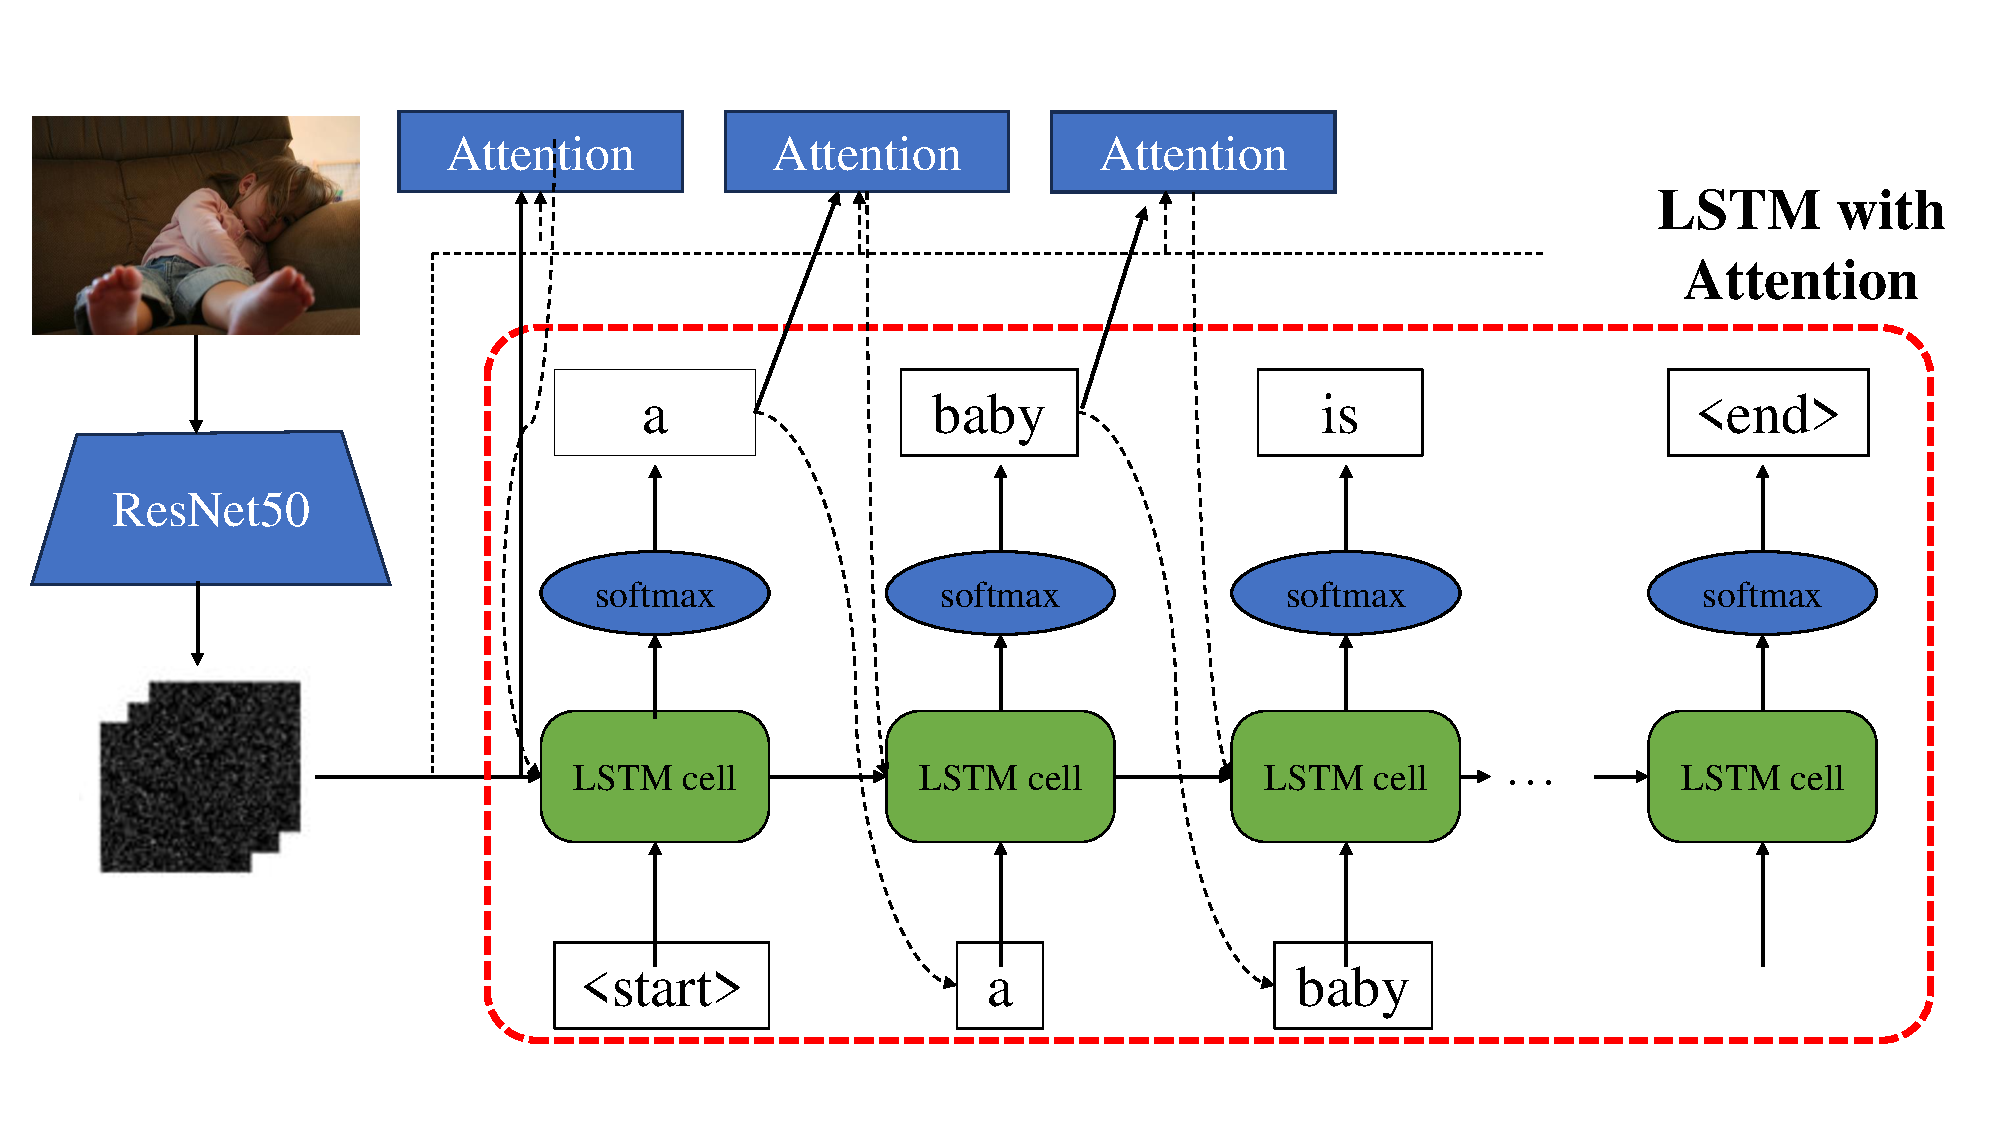
\includegraphics[width=0.7\textwidth]{assets/resnet50-lstm-attention.pdf}
  \caption{ResNet50 - LSTM - Attention architecture for image captioning}
  \label{fig:CNN_LSTM_Attention}
\end{figure*}


% TODO: Chỉnh sửa lại cho phù hợp
a) Encoder: A convolutional neural network (CNN) responsible for extracting features from the input image. The CNN outputs a fixed-size feature vector that represents the image.


b) Attention Mechanism: This component assigns weights to image features to indicate their importance. The attention mechanism allows the model to focus on the relevant regions of the image during the caption-generation process. Specifically, the model employs a soft attention mechanism to establish a correlation between the image features and each word in the caption.


c) Decoder: A recurrent neural network (RNN), specifically a Long Short-Term Memory (LSTM) network, uses the output of the CNN as input. LSTM generates each word in the caption based on the previous input and information from the image.


\subsection{Encoder: Convolutional Neural Networks\label{subsec:encoder}}
% Giới thiệu CNN trong vai trò encoder
% Vì cần làm gọn lại nên có bỏ một số phần
Convolutional Neural Networks (CNNs) are widely employed as encoders for image captioning tasks. The CNN architecture allows hierarchical feature learning through convolutional operations, which capture local patterns and gradually aggregate them to form higher-level representations. The CNN model is a feedforward neural network in which layers are interconnected through convolution operations. 


% Bỏ bớt phần này / hoặc viết gọn lại
% Một lớp trong mạng CNN có thể là Convolutional layer, Pooling layer hoặc Fully connected layer. Convolutonal layer là layer chứa các filter tương tự như hidden units và output được tính bằng cách thực hiện phép convolution với đầu vào và sử dụng activation function. Pooling layer được sử dụng để giảm số chiều của ma trận, nhờ đó giảm số tham số để tính cho layer tiếp theo, có 2 loại thường sử dụng là lấy trung bình của một vùng (average) hoặc lấy giá trị lớn nhất trong một vùng (max) với kích thước cho trước. Fully connected layer là một layer chứa các neuron như mạng neuron nhân tạo truyền thống, nhận vào một vector và trả ra vector mới, vì vậy ma trận trước khi đưa vào Fully connected layer sẽ được trải phẳng ra trước, lúc đó vector sẽ có kích thước $n=n_{H}*n_{W}*n_{C}$. Hàm kích hoạt phổ biến nhất cho mạng CNN là hàm ReLU (rectified linear unit), có công thức là:
% $$f(x)=max(0,x)$$
% giúp cho việc tính toán nhanh hơn và tốc độ hội tụ nhanh hơn. Hình \ref{fig:CNN_architecture} thể hiện một mô hình CNN đơn giản.


% Trong bài này sử dụng Resnet50, giới thiệu Resnet50
A common issue in CNN is the vanishing gradient problem, which can hinder the training process and limit the network's ability to learn effectively. The depth of the network is crucial for neural networks, but deeper networks are more difficult to train. To address this challenge, we decide to use the ResNet50 \cite{he2015deep}.
% TODO: dùng từ decide phù hợp không?


% Giới thiệu residual block
ResNet\cite{wang2017residual} introduces the concept of residual blocks, which enable the network to learn identity mapping. The residual block architecture is illustrated in Fig. \ref{fig:residual_block}. These residual blocks allow the model to skip connections and propagate information more effectively through the network, thereby mitigating the vanishing-gradient problem. This approach not only boosts the model's performance but also helps accelerate convergence during training.


% Trong bài này, nhóm sử dụng một loại mô hình CNN có tên gọi là ResNet-50\cite{he2015deep}. Đây là một mô hình gồm 50 lớp và có thể giải quyết hiện tượng \textit{Vanishing Gradient} khi xây dựng mạng CNN bằng cách sử dụng các \textit{Residual block}, minh họa Residual block so với khối bình thường như ở hình \ref{fig:residual_block}. Với residual block, input có thể lan truyền xuôi (forward propagate) nhanh hơn thông qua các residual connections (việc đưa input x vào phép tính tổng như hình \ref{fig:residual_block}) ở các layer. Hình \ref{fig:resnet_architecture} thể hiện chi tiết kiến trúc của mô hình ResNet với số layer tương ứng \cite{he2015deep}.



This model produces a set of feature vectors, specifically L vectors, where each vector belongs to the $R^D$ space, representing different parts within an image. To extract these feature vectors from the layers, the CNN model eliminates Fully Connected layers, which are typically used for object classification tasks.


\begin{figure}[h]
    \centering
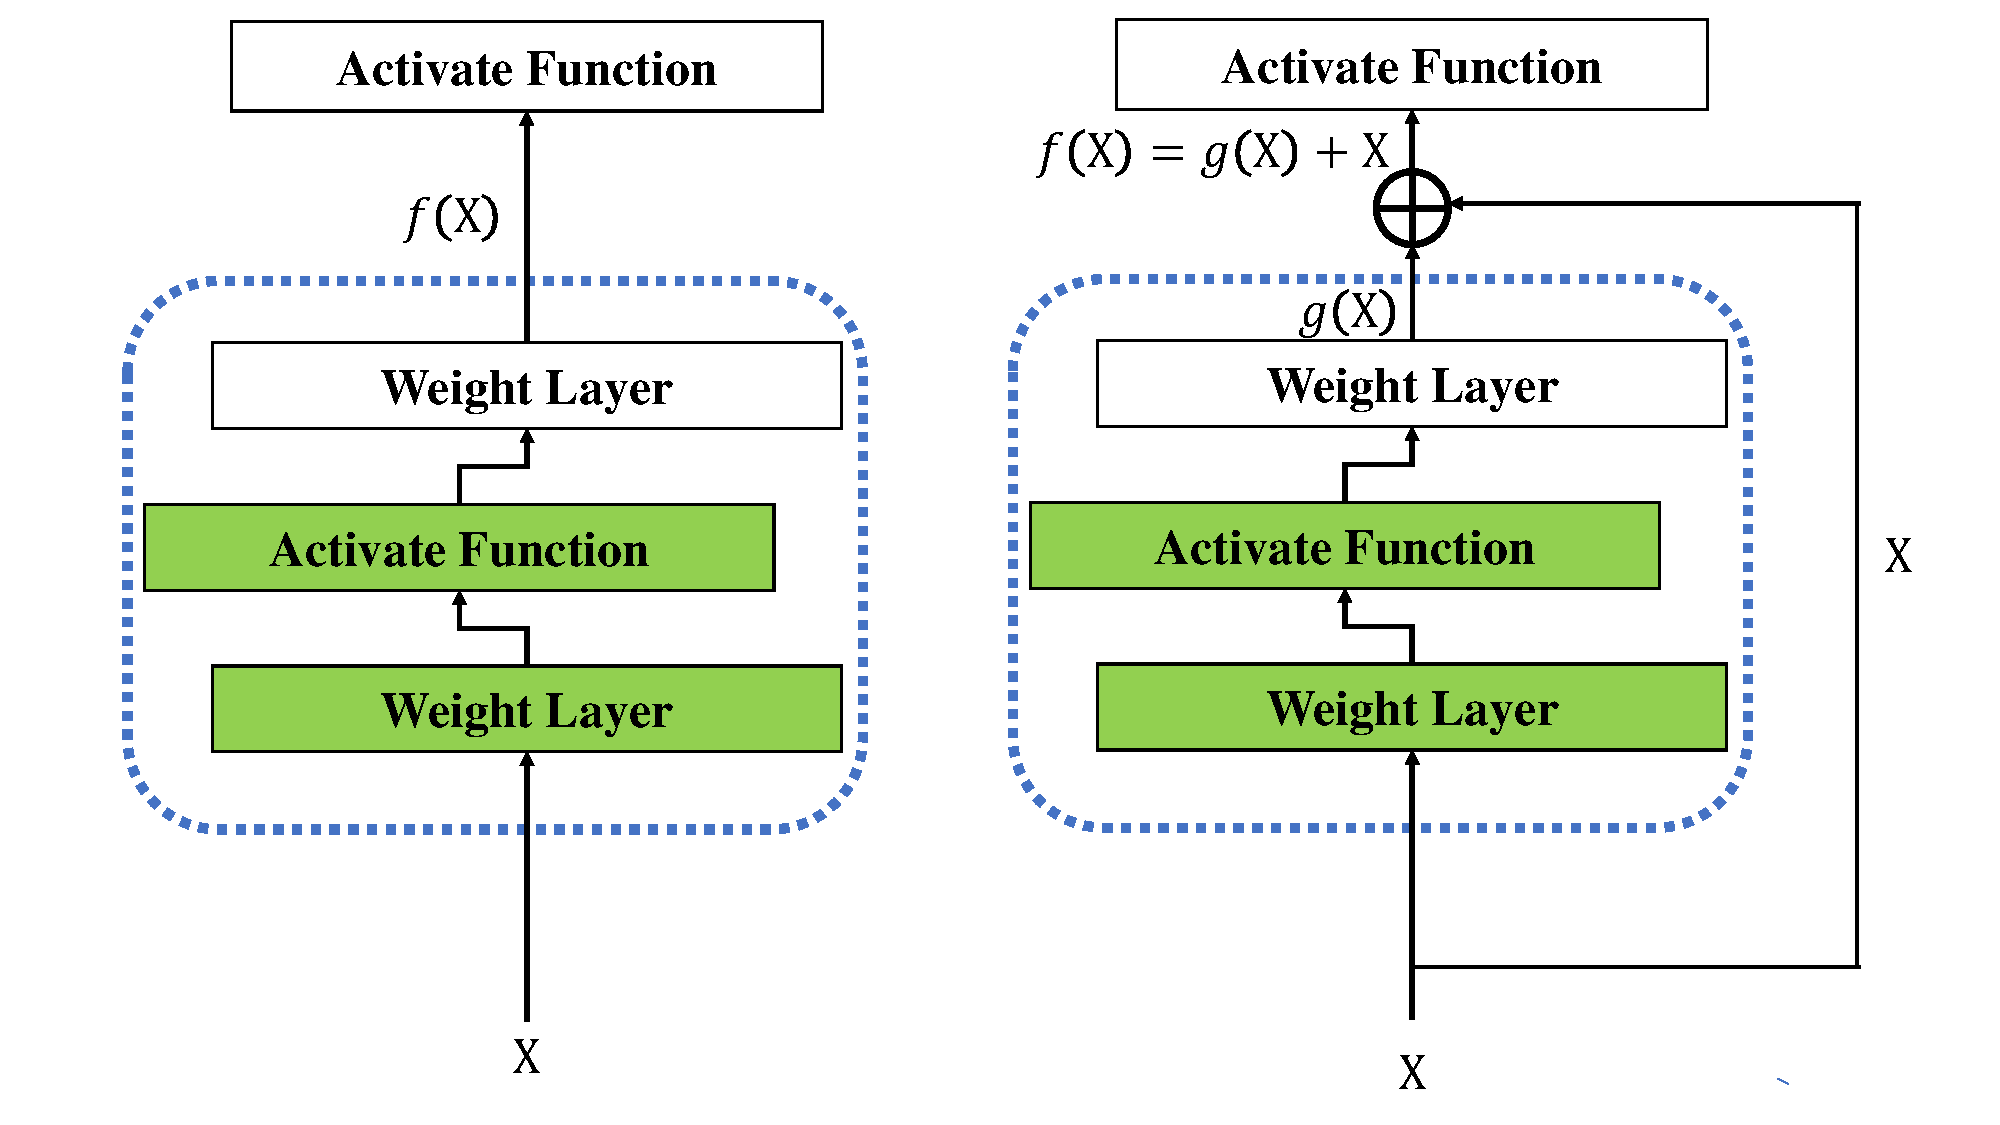
\includegraphics[width=\columnwidth]{assets/residual_block.pdf}
  \caption{Different between regular block (left) and residual block (right) (Source: adapted from \cite{jafar2021high})}
  \label{fig:residual_block}
\end{figure}


% Mô hình này sẽ tạo ra một tập hợp các vector thể hiện đặc trưng, cụ thể là L vector và với mỗi vector thuộc không gian $R^D$ thể hiện các phần trong ảnh. Để có thể trích xuất được vector đặc trưng từ layer, mô hình CNN sẽ bị bỏ bớt các Fully connected layer vì đây là những layer sử dụng để cho bài toán phân loại đối tượng. 


\subsection{Decoder: Long Short-term Memory Network\label{subsec:decoder}}
% TODO: cần chỉnh sửa lại nguyên phần này sau


% Thường dùng RNN làm decoder, tuy nhiên nó gặp vấn đề đạo hàm. nên thay bằng LSTM
The decoder generates captions for each word based on the features extracted by the encoder. Recurrent Neural Networks (RNNs) are suitable for this task. However, traditional RNNs encounter challenges, such as vanishing and exploding gradient problems. To overcome these issues, Long Short-Term Memory Networks (LSTMs) \cite{hochreiter1997long} have been employed.

\begin{figure}[h]
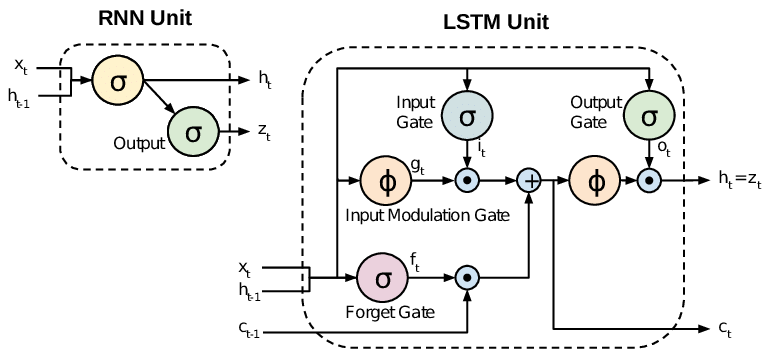
\includegraphics[width=\columnwidth]{assets/rnnvslstm.png}
  \caption{ Diagram of a basic RNN cell (left) and an LSTM memory cell (right) (Source: \cite{DBLP:journals/corr/RassemES17})}
  \label{fig:RNN_LSTM_compare}
\end{figure}


% Giới thiệu LSTM
LSTM offers an effective solution by introducing a specialized structure known as the LSTM cell, which incorporates forget gates to control information flow. These forget gates enable the LSTM to retain relevant information from the previous time steps while discarding irrelevant information. This mechanism ensures that the gradients are more stable during backpropagation, allowing the LSTM to effectively capture long-range dependencies and improve the quality of the generated captions.


An LSTM unit has a more complex structure than an RNN unit. It utilizes gated mechanisms, known as forget gates, to control information flow. Thus, LSTM can selectively retain information. LSTM can effectively store and recall information over long periods, enabling it to learn long-range dependencies.


The formula for updating the cell state at time t in an LSTM unit is as follows:

$$
\begin{pmatrix}
i \\f \\o \\g
\end{pmatrix}
= 
\begin{pmatrix}
\sigma \\ \sigma \\ \sigma \\ tanh
\end{pmatrix}
\circ
W
\begin{pmatrix}
h_{t-1} \\
x
\end{pmatrix}
$$
$$
c_t = f\circ c_{t-1} + i\circ g
$$
$$
h_t = o \circ tanh(c_t)
$$
$$
p_t = softmax(h_t)
$$
where, $\sigma$ is the sigmoid function. i, f, o, c, h are the input, forget, output, memory, hidden states. $p_t$ is the probability distribution for all the words. The word with the highest probability is chosen at each step and included in the next step to form a sentence.

% Trong đó, $\sigma$ là hàm sigmoid, i, f, o, g là các cổng quên, với $p_t$ là phân phối xác suất với tất cả các từ. Từ có xác suất lớn nhất được chọn ở từng bước và sẽ được đưa vào bước tiếp theo để tạo thành câu. 


% Bỏ hình RNN - Xài chung hình LSTM
% \begin{figure}[h]
% 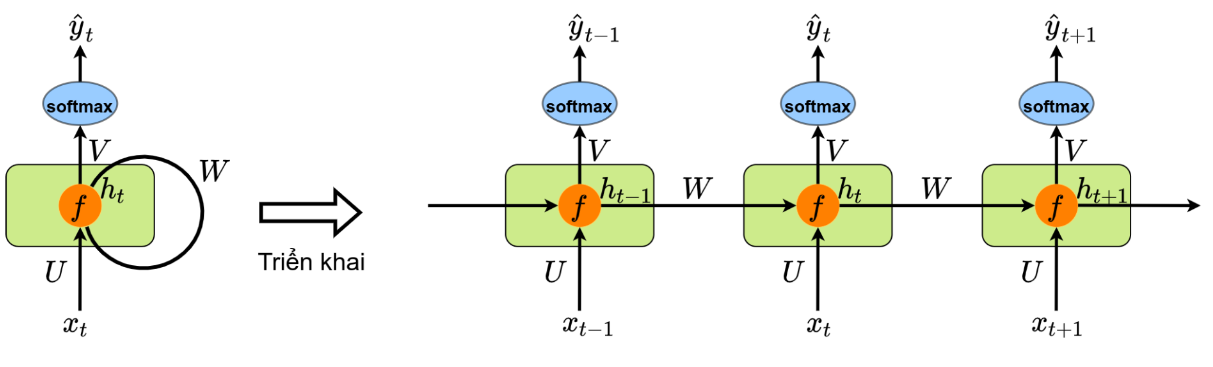
\includegraphics[width=0.5\textwidth]{assets/RNN_model.png}
%   \caption{Minh họa kiến trúc RNN}
%   \label{fig:RNN_architecture}
% \end{figure}




% Trong bài toán image captioning, sử dụng LSTM làm bộ giải mã là lựa chọn phổ biến và hiệu quả.
% LSTM cho phép mô hình học các mẫu ngôn ngữ phức tạp, xử lý thông tin từ ảnh và tạo ra các từ dự đoán phù hợp.
% Đồng thời, LSTM cũng giúp mô hình duy trì trạng thái ẩn và ghi nhớ thông tin quan trọng từ các từ đã sinh ra trước đó, tạo nên sự liên kết và logic trong câu chú thích.



\subsection{Attention Mechanism\label{subsec:attention}}


% TODO: xem xét bỏ hình này
% \begin{figure*}[t]
% \centering
% 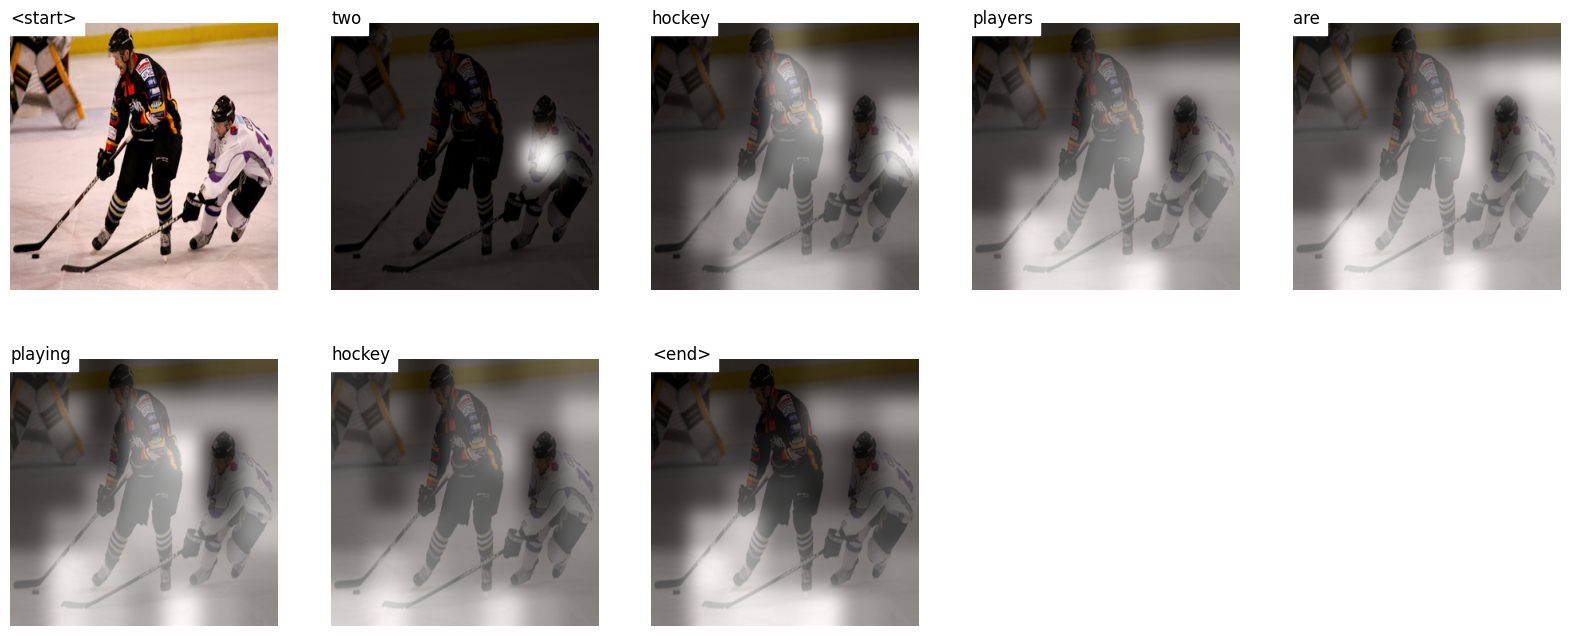
\includegraphics[width=\textwidth]{assets/attention.png}
%   \caption{Minh họa vùng ảnh mà mô hình tập trung vào trong quá trình phát sinh câu mô tả. Những vùng ảnh được quan tâm sẽ sáng hơn phần còn lại.}
%   \label{fig:RNN_LSTM_attention}
% \end{figure*}


% Hạn chế của không attention
The current CNN-LSTM model is limited in that it only provides image content once, specifically at the initial step of the LSTM, attempting to decode the entire image from the last hidden state $h_0$. While one approach to addressing this limitation involves feeding the entire image information % TODO: Dùng từ "image information" có phù hợp không?
at each step, this method leads to computational inefficiency.


% Giới thiệu soft attention
A more effective solution is to focus selectively on important regions within an image by employing a soft attention mechanism \cite{mcclenny2020self}. Soft attention has been extensively used in image classification tasks \cite{wang2017residual} % TODO: cite này đúng không?
because it allows the model to assign weights based on the significance of different regions. The soft attention mechanism is incorporated by adding an attention gate to the LSTM, enabling the model to concentrate its attention selectively, as shown in Figure \ref{fig:CNN_LSTM_Attention}.


% Công thức
% TODO: đọc phần này kì lắm luôn
The new formula for updating the cell state at time t is as follow:

$$
\begin{pmatrix}
i \\f \\o \\g \\\alpha_t
\end{pmatrix}
= 
\begin{pmatrix}
\sigma \\ \sigma \\ \sigma \\ tanh \\ softmax
\end{pmatrix}
\circ
W
\begin{pmatrix}
I \circ \alpha_{t-1} \\ h_{t-1} \\ x
\end{pmatrix}
$$
where, $\alpha_t$ is an attention vector at time t.

By using the softmax function, we ensure that each $\alpha_t>0$ for every pixel and for a vector containing all pixels, $\sum{}{}\alpha_t=1$. Soft attention is differentiable and can be trained using a standard backpropagation algorithm.


To calculate the specific value of $\alpha_t$ for each position $i$, \cite{xu2015show} presents the following equations:
$$e_{ti}=f_{att}(a_{i},h_{t-1})$$
$$\alpha_{ti}=\frac{exp(e_{ti})}{\sum_{k=1}^{L} exp(e_{tk})}$$
where, $f_{att}$ is the attention model that uses a multilayer feedforward neural network, $\alpha_{i}$ represents the degree of focus placed on the position of the model. Subsequently, the context vector $\hat{z_{t}}$ is computed as follows:
$$\hat{z_{t}}=\sum_{i=1}^{L} \alpha_{ti}a_{i}$$


The loss function used in the training process is:
$$L=-\log (P(y|x)) + \lambda \sum_{i}^{L} (1-\sum_{t}^{C} \alpha_{ti})^2$$


\subsection{Word embedding\label{subsec:embedding}}
\subsubsection{GLoVe Embeddings}
GLoVe (Global Vectors for word representation)\cite{pennington2014GLoVe} is an unsupervised method for obtaining vector representations of words based on the statistics of the co-occurrence of word pairs in a corpus. It combines the benefits of two main model families: global matrix factorization and local context window methods. Therefore, it can produce high-quality word vectors for use in downstream tasks. 

\subsubsection{fastText}  
fastText\footnote{Available at \url{https://github.com/facebookresearch/fastText}} provides two efficient word representation learning models based on the skipgram model and the continuous bag-of-words (CBOW) model\cite{mikolov2013efficient}. These models have been optimized to generate superior word representations by taking advantage of subword information and position weights. The skip-gram model with subword information is introduced in \cite{bojanowski2017enriching}, each word is decomposed into its character ngrams and word vectors are the sum of its character ngrams vector representations. The usage of position weights in the CBOW model is introduced in \cite{mnih2013learning}, each word vector is element-wise multiplied by a position-dependent vector.   



\section{Experiments\label{sec:experiment}}
\subsection{Training Procedure\label{implement}}
% TODO: viết gọn lại, không cần giải thích hay giới thiệu khái niệm kĩ quá
Models were trained in Google Colaboratory, which provides a NVIDIA Tesla T4 GPU, an Intel Xeon CPU with 2 vCPUs (virtual CPUs), and 13GB of RAM for chargeless access. We used Pytorch to implement the code for these models.  

For preprocessing captions, we added four special tokens $<start>$, $<end>$ standing for the start of the sentence, the end of the sentence, $<unk>$ standing for words which appear less than five times, $<pad>$ standing for a pad in the sentence to make all sentences have the same length. Next, we built a vocabulary from captions in the dataset. For pretrained word embeddings, we just kept words that appear in the vocabulary. Images are preprocessed to use Pytorch pretrained models. The detail of the image preprocessing method is described in its weight documentation\footnote{\url{https://pytorch.org/vision/main/models.html}}. 

We used pretrained ResNet-50 model for encoder which was trained for 1.2 million images of the ImageNet dataset for classification task. Since the pretrained model was trained for classification task, we stripped last two layers to get 14x14x2048 feature map for each image. Subsequently, the LSTM model operates on the flattened 196x2048 encoder output to generate sentences. Each LSTM cell has 512 hidden elements. 

For training the model without pretrained word embedding, elements of word embedding matrix are randomly generated from a uniform distribution for easier convergence. For training two models with pretrained word embedding, we used value from pretrained word vectors for initial elements of word embedding matrix. Beam search size 5 was used to produce better captions.

Adam algorithm\cite{kingma2014adam} was used to optimize training process with initial learning rate $10^{-4}$ for encoder and $4\cdot10^{-4}$ for decoder. In addition, we applied dropout technique with a value of 0.5 in LSTM layers to help avoid overfitting. 

% TODO: tạo một subsecton Evaluate protocol
We trained the model in two stages. At the first stage, we trained only decoder with a batch size of 64 around 15 epochs. Next, we continued from the model has highest BLEU-4 score from the first stage allowing fine-tuning of the encoder with a batch size of 32 around five more epochs. We saved the model having highest BLEU-4 score during validation. 

\subsection{Dataset}
We evaluate the performance of the proposed model using the Flickr30k dataset \cite{jia2015guiding}. This dataset contains 31,000 images. Each image corresponds to five artificially generated descriptions. The images in this dataset are mainly related to humans involved in everyday activities and events.

We use the Karpathy split \cite{karpathy2015deep} to create the training, validation, and test sets. The numbers of images in the training, validation, and test set are 29000, 1000, and 1000, respectively. Each image has five captions provided by human annotators\cite{jia2015guiding}.


\subsection{Evaluation Metrics}
Unlike typical tasks, in the image captioning problem, in addition to evaluating the accuracy of the generated captions, it is essential to assess their coherence and grammatical correctness.


To evaluate the performance of the models, we use the following metrics: BLEU \cite{papineni2002bleu}, METEOR \cite{banerjee2005meteor}, and ROUGE-L.


BLEU: This widely used machine translation metric analyzes the co-occurrences of n-grams between candidate (generated) and reference (ground truth) sentences.


METEOR: Based on the harmonic average of the precision and recall, METEOR addresses certain issues present in BLEU. This highly correlates with human discrimination based on recall.


ROUGE-L: This metric relies on the longest common subsequence (LCS) between generated and reference sentences. Higher quality summaries are determined by longer LCS. One drawback of this method is that it requires continuous n-grams.

\subsection{Pretrained word embeddings}
% TODO: không nên để link vô đây. để footnote đi
\subsubsection{GLoVe}We used pretrained 300-dimensional word vectors \footnote{Available at \url{https://nlp.stanford.edu/projects/GLoVe/}} which are trained on the combination of 2014 Wikipedia and Gigaword 5 with total of 6 billion tokens and a vocabulary of the top 400,000 most frequently occurring words using the GLoVe model\cite{pennington2014GLoVe}. 
\subsubsection{fastText}We used pretrained 300-dimensional English word vectors provided by \cite{grave2018learning}, which are trained on Common Crawl and Wikipedia using fastText. The model was trained CBOW with position-weights, with character n-grams of length 5, a window of size 5 and 10 negatives. 


\subsection{Results and Discussion\label{res}}

\subsubsection{Quantitative Results} \hfill % trick for enter newline, khong xoa dong trong duoi kia

First, we initiated a comparison between the model using word embeddings trained from scratch and the models utilizing pretrained word embeddings. A graph illustrating the metric values for each training epoch on the validation dataset is shown in Fig. \ref{fig:compare_val_score}.

\begin{figure}[h]
    \centering
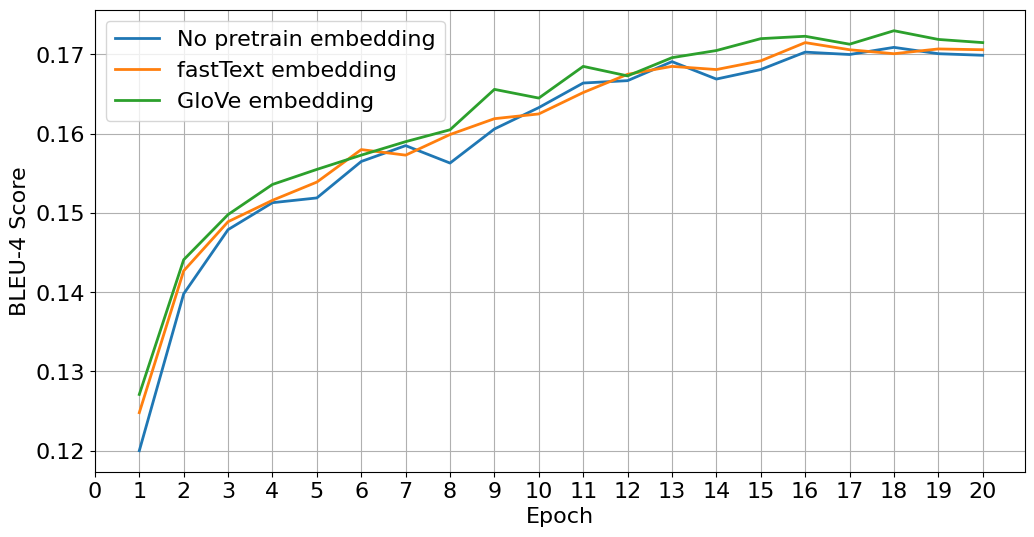
\includegraphics[width=\columnwidth]{assets/metric_compare_train_phase.png}
\caption{Validation of BLEU-4 score per epoch during training phase (20 first epochs) for model without pretrained embedding, model with fastText pretrained embedding, and model with GLoVe pretrained embedding.}
% TODO: '20 first epoch' sai ngu phap khong???
\label{fig:compare_val_score}
\end{figure}


% TODO: Dùng từ Model (tên cột) có phù hợp không?
\begin{table*}[h]
\centering
\caption{Performance of three models comparison in terms of BLEU-n (n = 1,2,3,4), METEOR, and ROUGE-L on the Flickr30k dataset. Bold numbers represent the best result for each metric.}
\label{tab:metric-compare-1}
\resizebox{0.7\textwidth}{!}{%
\begin{tabular}{l|rrrr|rr}
\cline{2-5}
 & \multicolumn{4}{c|}{\textbf{BLEU}} & \multicolumn{1}{l}{} & \multicolumn{1}{l}{} \\ \hline
\multicolumn{1}{|l|}{\textbf{Model}} & \multicolumn{1}{c|}{\textbf{BLEU-1}} & \multicolumn{1}{c|}{\textbf{BLEU-2}} & \multicolumn{1}{c|}{\textbf{BLEU-3}} & \multicolumn{1}{c|}{\textbf{BLEU-4}} & \multicolumn{1}{c|}{\textbf{METEOR}} & \multicolumn{1}{l|}{\textbf{ROUGE-L}} \\ \hline
\multicolumn{1}{|l|}{No pretrained} & 65.55 & 47.39 & 33.86 & 24.07 & \multicolumn{1}{r|}{19.51} & \multicolumn{1}{r|}{45.18} \\
\multicolumn{1}{|l|}{fastText} & 66.19 & 47.73 & 33.84 & 24.12 & \multicolumn{1}{r|}{19.50} & \multicolumn{1}{r|}{45.48} \\
\multicolumn{1}{|l|}{GLoVe} & \textbf{66.39} & \textbf{48.13} & \textbf{34.65} & \textbf{24.75} & \multicolumn{1}{r|}{\textbf{19.81}} & \multicolumn{1}{r|}{\textbf{46.27}} \\ \hline
\end{tabular}%
}
\end{table*}

\begin{figure*}[h]
\centering
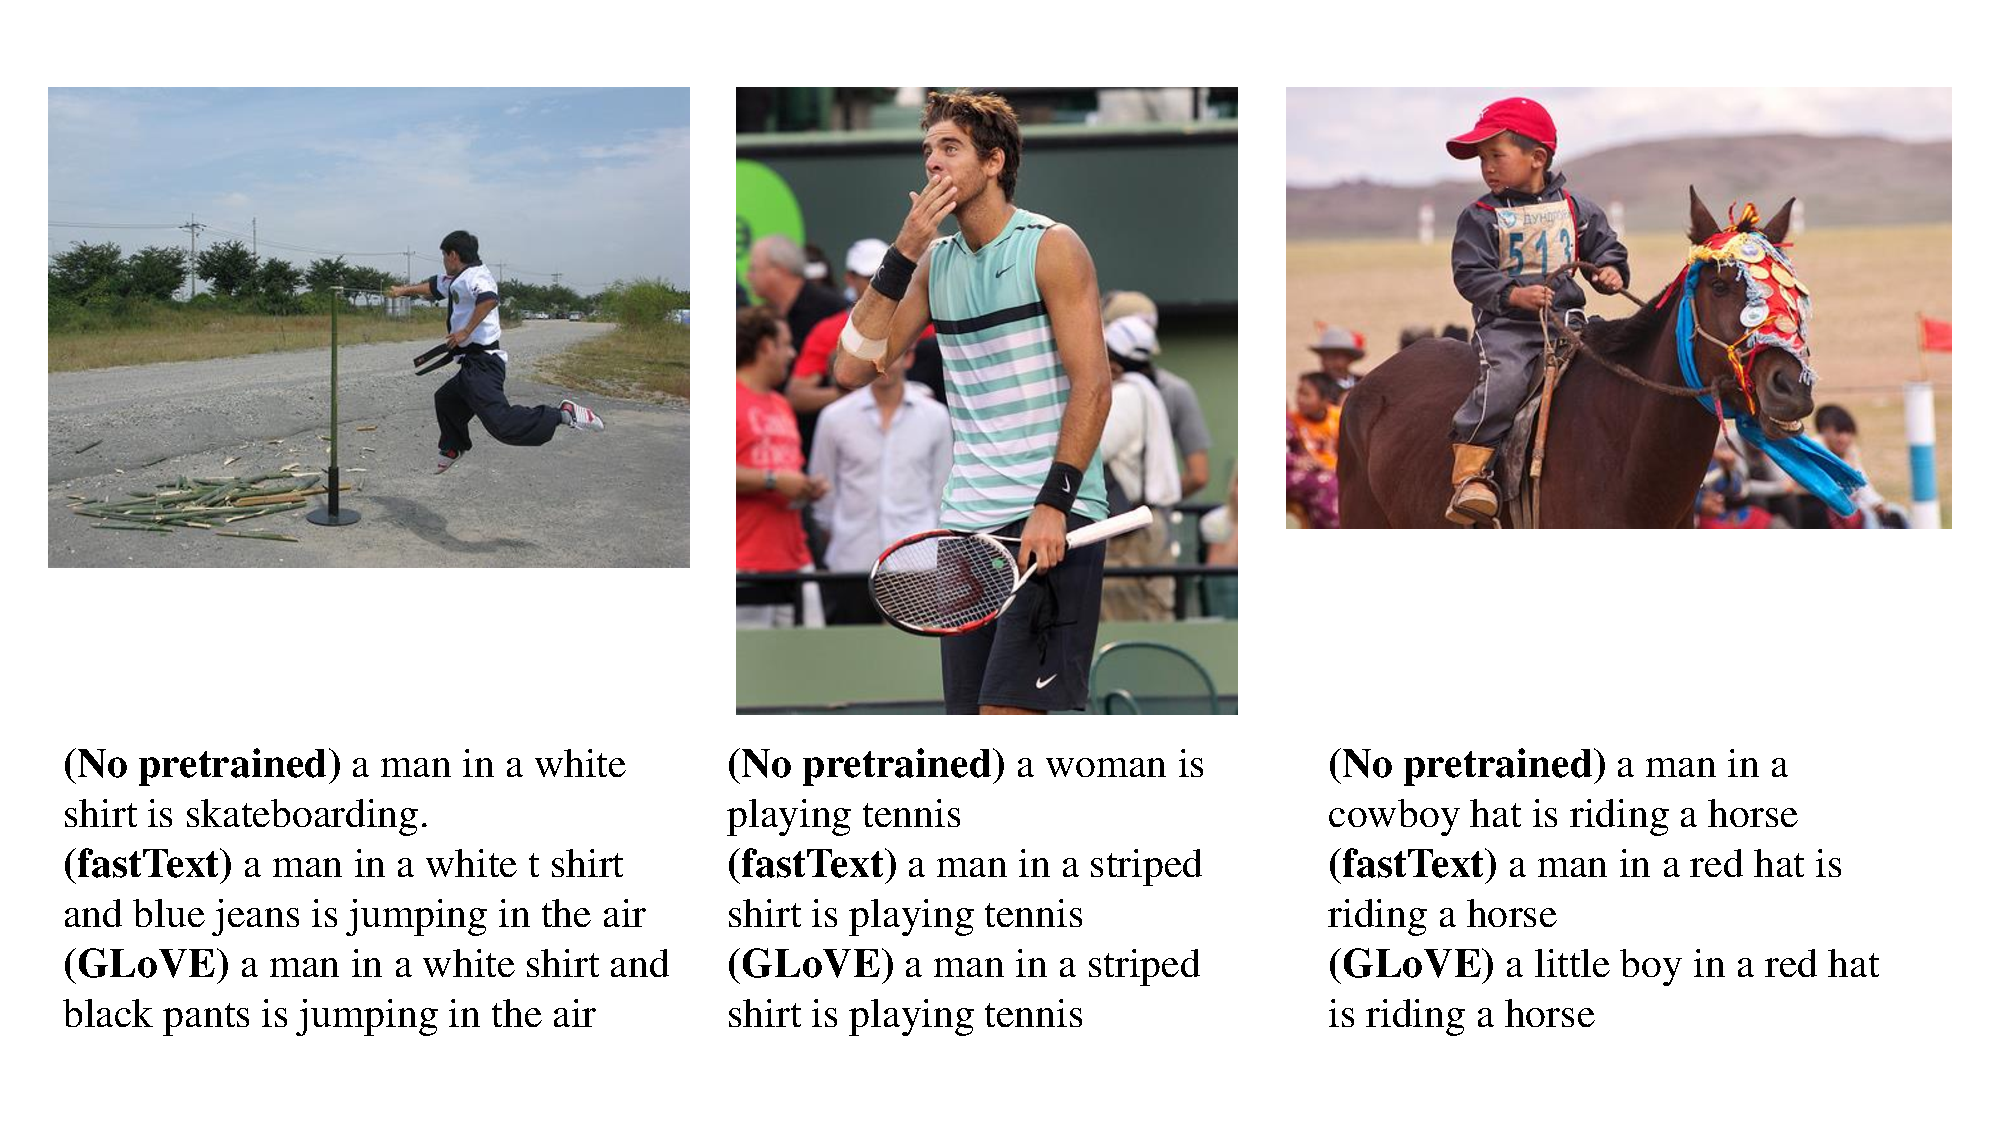
\includegraphics[width=0.85\textwidth]{assets/predict.pdf}
\caption{Examples of generated captions for given images. Each image has three captions, corresponding to a model that does not use pre-trained embedding, a model using fastText embedding, and a model using GloVE embedding.}
\label{fig:predict}
\end{figure*}


The results show that models using pretrained embeddings demonstrate significantly higher scores from the initial epoch. In contrast, the model without pretrained embeddings achieves a score of only 0.12 after the first training epoch, whereas the models with fastText and GLoVe pretrained embeddings achieve scores of 0.1248 and 0.1271, respectively. This disparity can be attributed to the fact that pretrained embeddings inherently carry substantial information about word semantics in the language, enabling the model to capitalize on this advantage from the outset.


As time progresses, the performance gap between models with pretrained embeddings and those trained from scratch diminishes, although models with pretrained embeddings still attain superior results.  For example, after the 20th epoch, the model without pretrained embeddings achieves a score of 0.1699, whereas the models with pretrained embeddings achieve scores of 0.1706 and 0.1715, respectively, for fastText and GLoVe embeddings.


Additionally, it is important to highlight that the model using GLoVe embeddings outperforms the model utilizing fastText embeddings. The highest-scoring model with fastText pretrained embeddings achieves a score of 0.1707, whereas the best model with GLoVe pretrained embeddings achieves a superior score of 0.1730.


The final results of the comparison between the three models for all metrics using the test dataset are summarized in Table \ref{tab:metric-compare-1}. The findings clearly demonstrate that models employing pretrained word embeddings consistently yield better performance than models trained from scratch. In particular, the model utilizing the GLoVe embeddings achieves the most impressive results. The use of pretrained GLoVe embeddings leads to notable improvements when compare with the performance of models without pretrained embeddings, with a 2.82\% boost in BLEU-4, 1.54\% in METEOR, and 2.41\% in ROUGE-L.


\subsubsection{Qualitative Results}\hfill


Figure \ref{fig:predict} shows three examples of the generated captions for the provided images. Clearly, models utilizing pretrained word embeddings deliver more accurate and natural sounding responses, resembling human-like descriptions. The results emphasize the superiority of GLoVe word embeddings over fastText in improving image captioning performance. 


% Chúng em đưa ra ví dụ dự đoán từ mô hình được huấn luyện trên tập dữ liệu Flickr30k ở hình \ref{fig:predict}. Dựa vào cơ chế tập trung, mô hình có thể nắm bắt và xác định được các chủ thể chính trong ảnh và đưa ra dự đoán khớp với trực quan của con người.

% Ở một vài trường hợp, mô hình đưa ra dự đoán đúng về chủ thể chính nhưng lại không đúng ở chủ thể khác xung quanh. Đối với một số mẫu phức tạp, có khả năng gây nhầm lẫn cao khiến cho mô hình đưa ra dự đoán sai. Tuy nhiên, nhờ vào cơ chế trực quan hóa những vùng mà mô hình tập trung vào để đưa ra quyết định (hình \ref{fig:RNN_LSTM_attention}), chúng em có thể hình dung được một cách trực quan lý do gây ra những sai lầm trong dự đoán của mô hình.


\section{Conclusion\label{conclusion}}
In this paper, we discussed the impact of using pretrained word embeddings on the results of the image captioning problem using BLEU, ROUGE-L, and METEOR metrics. The results of the experiment showed that pretrained word embeddings can improve the performance of the model. We found that using pretrained word embeddings with GLoVe yielded significantly better results. We hope that the results of this study will encourage further research on using word embeddings for other tasks in natural language processing. Furthermore, pre-trained word embeddings can be tested in other architectures, such as the object detection + CNN + LSTM approach.\cite{DBLP:journals/corr/YangZRH17}.

In future work, we will explore fine-tuning strategies for pretrained word embeddings, investigate multimodal embeddings, integrate attention mechanisms, and explore transfer-learning techniques. In addition, we will conduct fine-grained evaluations and test our model on larger, diverse datasets to assess its generalization capability. These efforts aim to enhance image captioning with efficient pretrained word embeddings and advance the field.


\renewcommand{\refname}{References}
\bibliographystyle{plain}
\bibliography{refs}

\end{document}
